
\chapter{\modif{Sur-segmentation adaptative par fusion de superpixels}}

\section{Introduction}

Ce chapitre présente un nouvel algorithme de sur-segmentation. Il s'agit du fruit d'une première réflexion, amorcée dans le but de concevoir une méthode de génération des superpixels capable d'améliorer les performances de $S \alpha F$. Au sein de $S \alpha F$, l'impact de la méthode de pré-traitement générant les superpixels est multiple. En particulier :
\begin{itemize}
\item la sur-segmentation est la seule des opérations travaillant au niveau du pixel : il s'agit donc de l'étape de $S \alpha F$ ayant la complexité algorithmique la plus élevée ;
\item les erreurs commises au niveau des superpixels ne peuvent pas être corrigées par la suite : l'algorithme de sur-segmentation a donc une influence forte sur la qualité du résultat produit par $S \alpha F$ ;
\item les superpixels étant utilisés comme primitives visuelles, ils déterminent en grande partie les caractéristiques des descripteurs employés pour différencier chacune des classes constituant la segmentation résultat.
\end{itemize}

Concrètement, qu'il s'agisse de l'adéquation de la segmentation produite avec la segmentation désirée, des temps d'exécution ou du nombre de germes demandés à l'utilisateur, tous les points sensibles de $S \alpha F$ dépendent d'une manière ou d'une autre des propriétés des superpixels générés. 


\subsection{Analyse des forces et faiblesses de SLIC}

Actuellement, $S \alpha F$ utilise l'algorithme SLIC \cite{achanta2012slic} proposé par Achanta \textit{et al.} L'un des principaux attraits de SLIC tient dans sa complexité linéaire qui lui assure des temps d'exécution significativement en dessous de ceux des méthodes concurrentes.

L'algorithme SLIC souffre cependant de deux faiblesses :
\begin{itemize}
\item il s'adapte peu à la complexité interne de l'image ;
\item il crée des superpixels homogènes uniquement au sens de la couleur. 
\end{itemize}

Le premier désavantage est directement lié à la propriété d'adaptabilité décrite au chapitre 3 : le choix d'un nombre de superpixels pertinent par rapport au niveau de détail de la photographie est à la charge de l'utilisateur. En particulier, nous regrettons que SLIC ne soit pas capable de réduire le nombre de superpixels dans des zones homogènes telles que le ciel ou de l'augmenter pour s'assurer de sur-segmenter correctement même les détails les plus fins de l'image. Nous y perdons, tant en termes de temps d'exécution qu'en termes de qualité des segmentations générées par $S \alpha F$.

Le second désavantage nous limite essentiellement dans le choix du descripteur : les superpixels n'étant pas conçus pour contenir des variations de couleurs, il y a une très faible probabilité que ces derniers contiennent une information de texture suffisamment discriminante pour améliorer l'identification des classes.

En outre, le fait que SLIC ne groupe les pixels qu'en fonction de leur localisation et de leur couleur \modif{engendre} parfois des erreurs de sur-segmentation. Si nous prenons par exemple l'image de la figure \ref{fig:asari:slic} et que nous cherchons à la sur-segmenter en superpixels dont l'aire moyenne est d'environ $300$ pixels, nous constatons que l'algorithme se trompe de manière suprenante, en intégrant dans un même superpixel des pixels de l'herbe et des pixels du zèbre. Ces aberrations s'expliquent par le fait que certaines rayures du zèbre sont plus petites que l'aire moyenne d'un superpixel : comme les pixels blancs n'ont, au sens de la couleur, aucune raison d'être regroupés avec des pixels noirs, ils sont rattachés à un ensemble regroupant d'autres pixels blancs, proche en termes de localisation, \modif{alors même que les deux ensembles ne sont pas voisins et que leur union ne forme pas une composante connexe}.

\begin{figure}[htb]
    \centering
    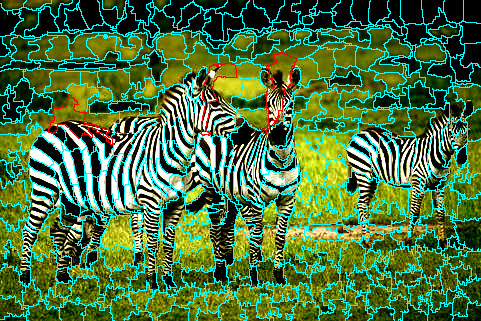
\includegraphics[width=0.6\textwidth]{images/asari/ex_slic}
    \caption{Exemple de superpixels (environ 500) produits par l'algorithme SLIC et comprenant des erreurs  introduites lors du post-traitement. Les contours des superpixels sont tracés en bleu. Les contours de certains superpixels erronés sont tracés en rouge. }
    \label{fig:asari:slic}
\end{figure}


Lors de la dernière étape de l'algorithme SLIC, ces ensembles se voient fragmentés en minuscules composantes connexes. Pour former des superpixels d'une taille moyenne proche de celle attendue, l'algorithme les fusionne avec des composantes connexes voisines, sans faire de vérification sur leur similarité au sens de la couleur. Ainsi, les rayures blanches peuvent se retrouver rattachées au rayures noires (créant l'illusion de superpixels texturés) ou bien à l'herbe, formant les superpixels erronés que nous observons.


\subsection{Démarche}

Les constats précédents nous ont conduit à travailler sur un nouvel algorithme, ASARI, de l'anglais \modif{ \og\emph{Adaptive Superpixel Algorithm with Rich Information}\fg} (algorithme de sur-segmentation adaptatif avec une information riche) \cite{mathieu2017asari}. Comme l'indique son nom, la première caractéristique d'ASARI consiste à s'adapter à la complexité de l'image, en réduisant le nombre de superpixels dans les zones uniformes de l'image.

La seconde spécificité d'ASARI réside dans le fait que, contrairement à SLIC, il produit des superpixels homogènes à la fois au sens de  la couleur et de la texture. À notre connaissance, la seule méthode de sur-segmentation à utiliser une information de texture est celle de Ren \textit{et al.} \cite{ren2003learning} dont les temps d'exécution importants \modif{en} freinent malheureusement l'utilisation. Avec ASARI, nous montrons qu'il est tout à fait possible d'avoir une méthode rapide bien que manipulant des caractéristiques de texture. 

Nous avons testé ASARI, à la \modif{fois selon} les protocoles de l'état de l'art \cite{achanta2012slic, stutz2015superpixel} et selon le protocole que nous proposons avec \modif{l'ensemble de données de référence HSID}. L'ensemble de ces tests montre qu'ASARI constitue un apport intéressant par rapport aux autres méthodes de sur-segmentation. Néanmoins, il doit encore faire l'objet d'adaptations avant de pouvoir être intégré fructueusement à $S \alpha F$.

\section{ASARI : un algorithme de sur-segmentation par fusion}
\label{sec:ASARI}

L'algorithme ASARI que nous \modif{proposons appartient} à la catégorie des méthodes de segmentation par fusion, formalisée pour la première fois en 2000, par Salembier \modif{\textit{et al.}} \cite{salembier2000binary}. Ce type d'algorithme sert de base, aujourd'hui encore, à un certain nombre de travaux fructueux en analyse d'image \cite{Li2016region,xu2016connected}.

Soit une image $I$  et un graphe \modif{$\mathcal{G}_{0}=\ <V_{0},E_{0}>$} la représentant, avec :
\begin{itemize}
\item $V_{0}$ un ensemble de sommets ;
\item  $E_{0}$ les arêtes qui les relient.
\end{itemize}
Les sommets de $V_{0}$ correspondent aux pixels de l'image ou bien à de petites régions. Les arêtes relient les sommets voisins. 

Un algorithme de segmentation par fusion appliqué sur le graphe initial $\mathcal{G}_{0}$ produit un graphe résultat $\mathcal{G}_{K}=\ <V_{K},E_{K}>$ tel que $V_{K}$ soit une partition de $V_{0}$ en composantes connexes et $E_{K}$ soit un sous-ensemble de $E_{0}$. 

Le passage de $\mathcal{G}_{0}$ à $\mathcal{G}_{K}$ s'effectue par la fusion des sommets de $V_{0}$ et la suppression des arêtes correspondantes. Salembier \textit{et al.} montrent qu'il existe une famille de méthodes dites de \emph{segmentation par fusion} assurant la production de $\mathcal{G}_{K}$. Ces méthodes respectent la procédure suivante :
\begin{itemize}
\item l'une des arêtes est sélectionnée ;
\item les deux sommets reliés par cette arête sont examinés ;
\item s'ils satisfont un critère dit \emph{de fusion} : 
\begin{itemize}
\item l'arête est supprimée ;
\item les deux sommets sont fusionnés en un seul sommet ;
\item les caractéristiques du nouveau sommet sont calculées.
\end{itemize}
\end{itemize}
Cette procédure est répétée jusqu'à qu'il n'existe plus d'arête reliant deux sommets qui peuvent être fusionnés. 

Ainsi, n'importe quel algorithme de segmentation par fusion se définit en donnant :
\begin{itemize}
\item un ordre de parcours, guidant la sélection des arêtes ;
\item un critère de fusion, indiquant si deux sommets doivent ou pas rester distincts ;
\item un modèle de \modif{région}, spécifiant comment les caractéristiques d'un nouveau sommet sont produites à partir de deux sommets fusionnés.
\end{itemize}

\subsection{Ordre de parcours }

L'ordre de parcours permet de déterminer quelles arêtes du graphe seront sélectionnées afin d'être éventuellement supprimées\footnote{Si l'algorithme autorise la fusion des deux sommets qu'elles relient.}. Dans le cas d'un algorithme standard de segmentation, l'ordre de parcours est généralement induit par une simple mesure de similarité, le but étant de créer des régions homogènes. Les régions produites correspondant aux objets présents dans l'image, il n'est pas choquant qu'elles soient de tailles différentes. 

L'une des particularités des algorithmes de sur-segmentation réside dans la contrainte supplémentaire de produire des régions de tailles relativement proches. L'ordre de parcours doit ainsi permettre une croissance homogène des régions en plus de garantir la sélection d'une arête ayant une probabilité raisonnable d'être supprimée.

Pour ce faire,  nous associons à chaque sommet $v_{i}$ un compteur $\Delta_{i}$ correspondant au nombre de fois où le sommet $v_{i}$ a été sélectionné. À chaque itération, l'algorithme choisit la région ayant la valeur $\Delta_{i}$ la plus faible.  En cas d'égalité entre plusieurs régions, l'une d'entre elles est sélectionnée de manière arbitraire.  Parmi l'ensemble des arêtes reliant $v_{i}$  à ses voisins, l'algorithme sélectionne celle qui maximise une mesure de similarité. Que $v_{i}$ soit fusionné ou pas, la valeur de $\Delta_{i}$ est incrémentée. 


\subsection{Mesure de similarité}
\label{sec:sim}

Afin de produire des superpixels qui ne soient pas uniquement homogènes au sens de la couleur, il est crucial qu'ASARI intègre une mesure de similarité au sens de la couleur et de la texture. Toutefois l'intégration d'une information visuelle plus riche ne doit pas faire perdre de vue la contrainte de rapidité qui pèse lourdement sur tous les algorithmes de sur-segmentation et se révèle particulièrement critique lorsque ces derniers sont intégrés à une méthode telle que $S \alpha F$. C'est donc en grande partie pour leur rapidité que nous avons choisi d'utiliser  les \emph{motifs ternaires locaux} (LTP, de l'anglais \og \emph{Local Ternary Pattern}\fg) \cite{tang2012topology}. 

\subsubsection{Descripteur de texture}
 Soient $p_{i}$ un pixel et $I(p_{i})$ son niveau de gris. La fonction seuil  \modif{$\mathcal{F}_{LTP}$} est définie par :\modif{
\begin{equation}
\mathcal{F}_{LTP}(p_{i},p_{j}) = \begin{cases}1, \text{ si } I(p_{i}) - I(p_{j}) > \omega_{LTP} \\
					0 \text{  sinon.}
\end{cases}
\end{equation}}
Le paramètre $\omega_{LTP}$ ajuste le comportement de la fonction.

Trouver le motif ternaire local de $p_{i}$ consiste à lui attribuer deux identifiants, $LTP_{N}$ et $LTP_{P}$, représentant les \modif{variations du niveau de gris dans} son voisinage. L'identifiant $LTP_{N}$ se construit à partir des voisins de $p_{i}$ ayant un niveau de gris significativement inférieur au sien, tandis que $LTP_{P}$ se calcule à partir de ceux ayant un niveau de gris significativement supérieur. 
 
 
Soit \modif{$\lbrace I(p_{i}^{0}), \cdots, I(p_{i}^{7})\rbrace$ les niveaux de gris 8 voisins de $p_{i}$}. L'identifiant $LTP_{N}$ est obtenu  grâce à la fonction  suivante : 
\modif{\begin{equation}
LTP_{N}(p_{i}) = \sum_{n=0}^{7} 2^{n} \mathcal{F}_{LTP}(I(p_{i}),I(p_{i}^{n})) \text{.}
\end{equation}}
Ainsi, pour que la fonction \modif{$\mathcal{F}_{LTP}$} soit égale à $1$, il faut que \modif{$I(p_{i}^{n})$} soit strictement inférieur à $I(p_{i})$ et que \modif{$|I(p_{i}) -I(p_{i}^{n})| > \omega_{LTP}$}.
 
De même, l'identifiant $LTP_{P}$ est obtenu  grâce à la fonction  suivante : 
\modif{\begin{equation}
LTP_{P}(p_{i}) = \sum_{n=0}^{7} 2^{n} \mathcal{F}_{LTP}(I(p_{i}^{n}),I(p_{n})) \text{.}
\end{equation}}
Ici, pour  que la fonction \modif{$\mathcal{F}_{LTP}$} soit égale à $1$, il faut que \modif{$I(p_{i}^{n})$} soit strictement supérieur à $I(p_{i})$ et que \modif{$|I(p_{i}) - I(p_{i}^{n})| > \omega_{LTP}$}.

\subsubsection{Détection des zones homogènes}
Les deux fonctions $LTP_{N}$ et $LTP_{P}$ sont des entiers compris dans l'intervalle $[0,255]$. Ces entiers peuvent être représentés sous la forme de nombres binaires à huit \modif{bits}. Le premier \modif{bit} correspond au résultat de la comparaison entre le pixel $p_{i}$ et son premier voisin, le deuxième au résultat de la comparaison avec le deuxième voisin, etc. 

Trois cas de figure peuvent se présenter :
\begin{enumerate}
\item le niveau de gris de $p_{i}$ est nettement inférieure à celui de son \modif{$k\ieme$} voisin  : dans ce cas, le \modif{$k\ieme$ bit} de l'identifiant $LTP_{N}$ est égal à $0$ et celui de l'identifiant $LTP_{P}$ est égal à $1$ ;
\item la valeur du niveau de gris de $p_{i}$ est nettement supérieure à celle de son \modif{$k\ieme$} voisin : dans ce cas, le \modif{$k\ieme$ bit} de l'identifiant $LTP_{N}$ est égal à $1$ et celui de l'identifiant $LTP_{P}$ est égal à $0$ ;
\item les deux niveaux de gris sont \modif{similaires}, c'est-à-dire que \modif{$|I(p_{i}) - I(p_{i}^{n})| \leq \omega_{LTP}$} : dans ce cas, le \modif{$k\ieme$ bit} de l'identifiant $LTP_{N}$  et celui de l'identifiant $LTP_{P}$ sont égaux à $0$.
\end{enumerate}

En particulier, si tous les voisins d'un pixel ont des niveaux de gris similaires au sien, les identifiants $LTP_{P}$ et $LTP_{N}$ valent tous les deux \modif{$0$}. Soit 
\begin{equation}
v_{i}^{0} = \lbrace p_{j} \in v_{i} \rbrace \text{, } LTP_{N}(p_{j})= LTP_{P}(p_{j})=0 \text{,}
\end{equation}
l'ensemble des pixels de la région $v_{i}$ ayant tout ses voisins avec des niveaux de gris similaires. 

Il est  aisé d'obtenir une estimation de la probabilité que la région $v_{i}$ soit \modif{non texturé}e en calculant :
\modif{\begin{equation}
P_{\neg T}(v_{i}) = \dfrac{|v_{i}^{0}|}{|v_{i}|}\text{, }
\end{equation}}
$|A|$ étant la cardinalité de l'ensemble $A$.

\subsubsection{Définition de la mesure de similarité}

Nous postulons que la mesure de similarité doit être faible lorsqu'elle compare une région \modif{non texturé}e avec une région texturée. Nous nous donnons les fonctions suivantes :
\begin{itemize}
\item \modif{$\mathcal{F}_{c}(i,j)$}, une mesure de similarité  au sens de la couleur entre les régions $v_{i}$ et $v_{j}$ ;
\item \modif{$\mathcal{F}_{t}(i,j)$}, une mesure de similarité au sens de la texture \modif{entre les régions $v_{i}$ et $v_{j}$ ;}
\item \modif{$\mathcal{F}_{h}(i)$}, une fonction binaire, valant $1$ si la région \modif{$v_{i}$} est \modif{non texturé}e, $0$ sinon.
\end{itemize}
\begin{emodif}
À partir de la probabilité $P_{\neg T}(v_{i})$ dont l'estimation est décrite précédemment, nous calculons :
\begin{equation}
\mathcal{F}_{h}(i)=\begin{cases} 
1 &\text{ si }  P_{\neg T}(v_{i}) > \omega_{T}\\
0 & \text{sinon.}
\end{cases}
\end{equation}
Le  paramètre $\omega_{T}$ correspond au seuil à partir duquel une région est considérée comme texturée.\end{emodif} Nous pouvons alors définir la fonction de similarité \modif{$\mathcal{F}_{S}$} comme : \modif{
\begin{equation}
\mathcal{F}_{S}(i,j) = \begin{cases} \mathcal{F}_{c}(i,j), &\text{ si } \mathcal{F}_{h}(i) + \mathcal{F}_{h}(j) = 2 \\
					\displaystyle\frac{\mathcal{F}_{t}(i,j) + \mathcal{F}_{c}(i,j)}{2},&\text{ si } \mathcal{F}_{h}(i) + \mathcal{F}_{h}(j) = 0 \\
					0 & \text{  sinon.}
\end{cases}
\end{equation}}

\subsubsection{Similarité au sens de la couleur}
Soit $v_{i}$ une région et  $c_{i}$ le vecteur de dimension $3$ contenant sa couleur. Le vecteur $c_{i}$ correspondant aux valeurs normalisées obtenues pour chacun des canaux d'un espace colorimétrique fixé. Une mesure de la similarité au sens de la couleur entre $v_{i}$ et $v_{j}$ est donnée par :
\modif{\begin{equation}
\mathcal{F}_{c}(i,j) = \exp(- \dfrac{1}{N_{c}}|| c_{i} - c_{j} ||)
\end{equation}}
avec $N_{c}$ le nombre de composantes pour la couleur (généralement $3$) et $||.||$ la norme euclidienne.

Nous avons testé les espaces \modif{RGB et Lab}. Ces deux espaces donnent des résultats similaires. L'espace Lab nécessitant des calculs intermédiaires pour convertir la couleur des pixels, nous avons privilégié l'utilisation de l'espace RGB durant l'évaluation d'ASARI.

\subsubsection{Similarité au sens de la texture}
Soit  $t_{i}$ la concaténation des histogrammes normalisés des deux identifiants $LTP_{N}$ et $LTP_{P}$, pour les pixels rattachés au sommet $v_{i}$. La mesure de similarité au sens de la texture utilisée par ASARI \modif{fait intervenir} la distance du $\chi^{2}$ entre les deux histogrammes :
\modif{\begin{equation}
\begin{split}
\mathcal{F}_{t}(i,j) &= \exp(- \chi^{2}(t_{i},t_{j}))\\
			 &=\exp \left( - \frac{1}{N_{t} }\sum_{k=0}^{N_{t}} \dfrac{{(t_{i}^{k} - t_{j}^{k} )}^{2}}{t_{i}^{k} + t_{j}^{k}} \right) \text{.}
\end{split}
\end{equation}}
La valeur $N_{t}$ correspond au nombre de classes ayant un nombre d’occurrences strictement positif, dans l'histogramme $t_{i}$ ou dans  l'histogramme $t_{j}$. 

\subsubsection{Temps d'exécution}

Distinguer les régions \modif{non texturé}es des régions texturées comporte deux avantages. D'une part, nous évitons de décrire uniquement par sa couleur moyenne une région dont la texture peut comporter des teintes très différentes. D'autre part, nous réduisons considérablement le temps d'exécution d'ASARI, la complexité de \modif{$\mathcal{F}_{c}$} étant très inférieure à celle de \modif{$\mathcal{F}_{t}$}. En effet, dans le premier cas, seules les trois composantes de couleur sont comparées, tandis que, dans le second cas\modif{,} il faut prendre en compte l'intégralité des éléments des histogrammes de $LTP$, soit $2\times256$ comparaisons. 

\subsection{Critère de fusion}
\label{sec:critfusion}

Dans le cas d'une méthode de segmentation, le critère de fusion se contente de garantir la cohérence de la région créée lorsque deux sommets sont fusionnés. Une méthode de sur-segmentation nécessite également de vérifier que la surface de la région obtenue ne soit pas disproportionnée par rapport à celles des autres régions. Ce contrôle s'ajoute à celui de l'ordre de parcours. 

Le critère de fusion d'ASARI est une fonction booléenne qui se décompose de la manière suivante : 
 \modif{\begin{equation}
\mathcal{F}_{F}(i,j) = \mathcal{F}_{F,S}(i,j) \land \mathcal{F}_{F,R}(i,j) \text{,}
\end{equation}}
avec \modif{$\mathcal{F}_{F,S}$} un critère prenant en compte la similarité et \modif{$\mathcal{F}_{F,R}$} un critère dépendant de l'aire de la nouvelle région. 

\subsubsection{Critère de similarité}
\label{subsec:asari:critSim}
La fonction booléenne \modif{$\mathcal{F}_{F,S}$} vérifie que la mesure de similarité entre les deux régions se situe au dessus d'un seuil :
\modif{\begin{equation}
\mathcal{F}_{F,S}(i,j) = \mathcal{F}_{S}(i,j) > \omega_{S}\text{.}
\end{equation}}

\subsubsection{Critère de régularité}
\label{subsec:asari:critReg}
La fonction booléenne \modif{$\mathcal{F}_{F,R}$} s'assure que la taille de la nouvelle région ne sera pas disproportionnée par rapport à celles des autres régions.

Soient \modif{$|v_{i}|$} le nombre de pixels appartenant à la région $v_{i}$ et $N_{V}$ le nombre de régions. La vérification effectuée est la suivante :\modif{
\begin{equation}
\mathcal{F}_{F,R}(i,j) = \left( (|v_{i}|+  |v_{j}|) < \dfrac{\omega_{R}}{N_{V}} \sum_{k=0}^{N_{V}-1} |v_{k}| \right)\text{.}
\end{equation}}
Le paramètre \modif{$\omega_{R}$} correspond à un \textit{a priori} sur la rapidité de croissance des régions : plus ce paramètre est élevé, plus la différence entre la taille de la nouvelle région et la taille des régions existantes est importante. Ainsi, si \modif{$\omega_{R}$} vaut $2$, l'aire de la nouvelle région ne devra pas dépasser le double de l'aire moyenne des régions existantes.

\section{Liens avec un problème d'optimisation}

\subsection{Reformulation sous la forme d'un problème d'optimisation}
Si nous convertissons le résultat booléen de la fonctions \modif{$\mathcal{F}_{F}$} en un résultat binaire égal à $0$ lorsque le prédicat n'est pas respecté et à $1$ lorsque l'arête doit être supprimée, nous constatons que l'algorithme ASARI revient à rechercher le graphe $\mathcal{G}_{K}^{*}$ permettant d'atteindre le minimum de la fonction :
\modif{\begin{equation}
\mathcal{F}_{ASARI}(\mathcal{G}_{K}) = \sum_{e_{i,j} \in E_{K}} \mathcal{F}_{F}(i,j)\text{.}
\end{equation}}

La fonction  \modif{$\mathcal{F}_{F}$} ne pouvant valoir que $0$ ou $1$, ce minimum vaut $0$\modif{, lorsque toutes les fusions ont été réalisées}. Comme les arêtes sont sélectionnées en fonction de la valeur du compteur $\Delta_{i}$, chaque sommet du graphe initial $\mathcal{G}_{0}$ est parcouru au moins une fois et l'une des arêtes le reliant à l'un de ses voisins est sélectionnée. Soit $N_{V_{0}}$ le nombre initial de sommets : dans le pire des cas, une seule fusion est réalisée et un parcours est relancé sur les $N_{V_{0}}-1$ sommets restants. Toujours dans le pire des cas, le processus se poursuit jusqu'à l'obtention d'un unique sommet. Dans ce cas de figure, la complexité d'ASARI vaut :\modif{
\begin{align}
O_{ASARI}&=N_{V_{0}} + (N_{V_{0}} -1) + \cdots + 1 \\
&=  \frac{N_{V_{0}}(N_{V_{0}}+1)}{2}\\
&=\dfrac{{N_{V_{0}}}^{2}+N_{V_{0}}}{2}\text{.}
\end{align}}

Même si ce cas de figure ne se produit en pratique jamais (il correspond à une fusion de l'ensemble des pixels en un seule région), il a le mérite de montrer qu'une implémentation naïve d'ASARI dépasse largement la complexité algorithmique tolérable pour un algorithme de sur-segmentation. 

Pour obtenir des temps d'exécution raisonnables et permettre à ASARI de passer à l'échelle, nous nous sommes contentés de rechercher une approximation de $\mathcal{G}_{K}^{*}$. En nous donnant un critère d'arrêt approprié et en réalisant une première étape d'initialisation permettant d'obtenir un graphe $\mathcal{G}_{1}$ tel que :
\modif{\begin{equation}
\mathcal{F}_{ASARI}(\mathcal{G}_{1}) > \mathcal{F}_{ASARI}(\mathcal{G}_{0})\text{,}
\end{equation}}
nous permettons à l'algorithme ASARI de produire rapidement une segmentation correcte.

\subsection{Critère d'arrêt}
De manière similaire à un algorithme de segmentation standard, ASARI s'arrête lorsque plus aucune arête ne peut être supprimée, \modif{c'est-à-dire} lorsque plus aucune paire de sommets ne satisfait le critère de fusion \modif{$\mathcal{F}_{F}$}. Au sein de ce critère, la fonction \modif{$\mathcal{F}_{F,S}$}  permet à l'algorithme de s'adapter à complexité de l'image : lorsque celle-ci contient de nombreux petits détails, elle arrête la fusion des régions, tandis que dans les zones homogènes, elle l'autorise, conduisant à de plus grands superpixels. En parallèle, la fonction \modif{$\mathcal{F}_{F,R}$}  arrête la fusion des régions avant que des disparités de taille trop importantes ne soient atteintes. 

Pour les raisons d'efficacité évoquées précédemment, il est également souhaitable d'arrêter l'algorithme lorsque tous les sommets ont été sélectionnés au moins $\omega_{Itr}$ fois et d'obtenir, non pas un résultat optimal mais une approximation. L'évaluation d'ASARI conduite dans la section~\ref{sec:res} montre que $\omega_{Itr}=10$ permet d'obtenir des résultats satisfaisants. 

Enfin, si le contexte applicatif nécessite qu'un nombre minimal de superpixels soit imposé, cette contrainte peut également être intégrée dans le critère de terminaison. 

\subsection{Initialisation}

 Afin de réduire les calculs nécessaires à ASARI, nous avons choisi de regrouper \modif{les pixels de l'image sur-segmentée} en petits ensembles connexes.

Le fait que les sommets de $V_{0}$ \modif{soient des} petites régions facilite également l'utilisation du descripteur de texture. En effet, ce dernier correspond à l'histogramme des deux identifiants $LTP_{P}$ et $LTP_{N}$ au sein de chaque région. Lorsque celle-ci ne contient qu'un très petit nombre de pixels (ou pire, un unique pixel), cet histogramme n'est pas exploitable. En nous assurant que les sommets de $V_{0}$ contiennent au moins une cinquantaine de pixels, nous évitons de manipuler des descripteurs de texture qui n'auraient pas de sens. 

Les régions donnant les sommets de $V_{0}$ sont obtenues avec l'algorithme SLIC \cite{achanta2012slic}, paramétré pour produire de tout petits superpixels. L'algorithme SLIC garantit une complexité linéaire par rapport au nombre de pixels, ce qui assure que l'obtention de $V_{0}$ n'augmente pas de manière drastique la complexité générale d'ASARI. De plus, le fait que SLIC soit paramétré pour produire de minuscules régions réduit considérablement le nombre d'itérations \modif{internes à SLIC qui sont} nécessaires à l'obtention d'une sur-segmentation, tout en garantissant un faible taux d'erreur de sous-segmentation. Durant l'ensemble de nos tests, trois itérations (\modif{au lieu d'une dizaine, lors d'une utilisation normale de SLIC})  se sont révélées suffisantes. 

L'inconvénient de cette approche est qu'elle introduit deux paramètres, $\omega_{V_{0}}$ et \modif{$\omega_{C}$} qui correspondent respectivement à la taille moyenne souhaitée pour les régions de $V_{0}$ et au paramètre de compacité de l'algorithme SLIC.

\section{Détermination des paramètres}
\label{sec:param}
L'algorithme ASARI comporte $6$ paramètres : 
\begin{itemize}
\item $\omega_{LTP}$ : le seuil permettant de décider si deux niveaux \modif{de gris} sont similaires ;
\item \modif{$\omega_{T}$} : un seuil au dessus duquel la probabilité d'une région d'être homogène est jugée suffisamment haute pour que cette dernière soit considérée comme non texturée ;
\item $\omega_{V_{0}}$ : l'aire moyenne souhaitée pour les régions de départ ;
\item \modif{$\omega_{C}$} : le paramètre de compacité de l'algorithme SLIC ;
\item \modif{$\omega_{S}$} : \modif{le paramètre du critère de similarité ;}
\item \modif{$\omega_{R}$} : le paramètre \modif{du critère de régularité.}
\end{itemize}

Comme ces paramètres ont une influence sur des aspects différents (nombre de superpixels, régularité, adhérence aux contours, etc.), il n'est pas aisé de les optimiser en une seule fois, de manière à maximiser un score de réussite. Nous avons choisi de procéder en trois étapes successives : optimisation de la détection des zones \modif{non texturé}es, paramétrage de SLIC et détermination des paramètres du critère de fusion. 

 L'évaluation menée dans la section \ref{sec:res} montre  qu'une fois ces paramètres fixés, ils permettent d'obtenir de bons résultats sur des photographies couleur ou noir et blanc, prises à l'extérieur ou à l'intérieur, de  tailles et de complexités variées. Les étapes d'apprentissage \modif{des paramètres} détaillées dans cette section n'ont donc pas besoin d'être répétées.

\subsection{Détection des zones \modif{non texturé}es}
Comme expliqué dans la section \ref{sec:ASARI}, la détection des zones \modif{non texturé}es est effectuée via les LTP, tout d'abord en détectant les pixels ayant un voisinage \modif{non texturé}, ensuite en repérant les régions composées en majorité de tels pixels. Deux paramètres doivent donc être fixés : $ \omega_{LTP} \in \left[0,255\right]$, le seuil à partir duquel les niveaux de gris de deux pixels sont considérés comme similaires et \modif{$\omega_{T} \in [0,1]$} la proportion de pixels avec un voisinage \modif{non texturé}, à partir de laquelle une région est considérée comme \modif{non texturé}e. 

Nous avons constitué un ensemble de $100$ images de $100\times100$ pixels, la moitié correspondant à des zones \modif{non texturé}es, le reste correspondant à des zones texturées. Ces images sont des patchs extraits d'images de la base de données de Wikimedia Commons\footnote{\url{https://commons.wikimedia.org/wiki/Accueil}} ainsi que de la base de données de Brodatz\footnote{\url{http://sipi.usc.edu/database/database.php?volume=textures}}. La figure \ref{fig:bddetecsmooth} montre quelques exemples d'images utilisées durant les tests. 

\begin{figure}[htb]
    \centering
    \begin{subfigure}[t]{0.45\textwidth}
        \centering
        
\includegraphics[width=0.3\textwidth]{images/asari/LTP/patch_l1}
        
\includegraphics[width=0.3\textwidth]{images/asari/LTP/patch_l2}
        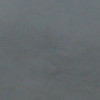
\includegraphics[width=0.3\textwidth]{images/asari/LTP/patch_l3}
        \caption{Exemples d'images correspondant à des zones \modif{non texturé}es.}
    \end{subfigure}%
    \\
    \begin{subfigure}[t]{0.45\textwidth}
        \centering
        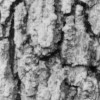
\includegraphics[width=0.3\textwidth]{images/asari/LTP/patch_nl1}
        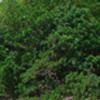
\includegraphics[width=0.3\textwidth]{images/asari/LTP/patch_nl2}
        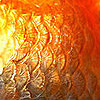
\includegraphics[width=0.3\textwidth]{images/asari/LTP/patch_nl3}
        \caption{Exemples d'images correspondant à des zones texturées }
    \end{subfigure}
    \caption{Exemples d'images utilisées pour le paramétrage de la détection des zones \modif{non texturé}es.}
    \label{fig:bddetecsmooth}
\end{figure}


À partir de ce jeu de données,  nous nous sommes ensuite ramenés à un problème de classification à deux classes :
\begin{itemize}
\item \emph{image texturée} ;
\item \emph{image \modif{non texturé}e}.
\end{itemize}
\modif{Soient} :
\begin{itemize}
\item $R_{t}$ l'ensemble des images texturées ;
\item $R_{h}$ l'ensemble des images \modif{non texturé}es ;
\item $C_{t}$ l'ensemble des images classées comme texturées ;
\item $C_{h}$ l'ensemble des images classées comme \modif{non texturé}es.
\end{itemize}
Nous avons cherché le couple $(\omega_{LTP},\omega_{T})$ permettant de maximiser le score de précision  :
\modif{\begin{equation}
\mathcal{F}_{P} =  \frac{|R_{t} \cap C_{t} |}{|C_{t}|} + \frac{|R_{h} \cap C_{h} |}{|C_{h}|}\textit{.}
\end{equation}}
Le paramètre $\omega_{LTP}$  étant un nombre \modif{entier} dans un intervalle borné, nous avons testé toutes les valeurs possibles. Pour \modif{$\omega_{T}$}\modif{,} nous avons choisi un pas de $\nombre{0,01}$. 
Les valeurs retenues sont de $12$ pour $\omega_{LTP}$  et de $\nombre{0,85}$ pour \modif{$\omega_{T}$}.

\subsection{Paramètres de SLIC }
Les résultats obtenus par la méthode SLIC \cite{achanta2012slic,stutz2015superpixel} montrent qu'une valeur de $10$ pour le paramètre de compacité assure une forme régulière des régions, proche du rectangle, tout en conservant une bonne adhérence aux contours. Nous avons donc conservé cette valeur pour \modif{$\omega_{C}$}. 

Le paramètre $\omega_{V_{0}}$ fixe la taille des régions de départ. Il est donc nécessaire qu'il soit inférieur à l'aire en pixels du plus petit objet d'intérêt. Il doit également permettre de produire des régions suffisamment grandes pour que le calcul de la probabilité qu'elles soient texturées ait du sens. Nous recommandons de ne pas fixer la valeur de ce paramètre en dessous de $50$ pixels. Si aucun \textit{a priori} n'est émis sur la taille du plus petit objet d'intérêt, une valeur entre $50$ et $150$ pixels permet d'obtenir des résultats satisfaisants pour une grande variété d'images. 

\subsection{Paramètres du critère de fusion}

Le paramètre \modif{$\omega_{S}$} correspond à la similarité minimale requise pour fusionner deux régions. Nous avons essayé de déterminer automatiquement ce seuil à partir des distances entre les superpixels. Il est par exemple possible de supposer que les sommets de $V_{0}$ peuvent\modif{,} pour la majorité\modif{,} être fusionnés avec le sommet voisin le plus proche (au sens d'un critère de similarité), d'analyser la distribution \modif{de la mesure} de similarité entre chaque sommet et son voisin le plus proche, en cherchant les modes de l'histogramme. 

Malheureusement, cette analyse statistique se révèle coûteuse, allant jusqu'à multiplier par trois les temps de calcul nécessaires à l'étape d'initialisation. Bien que n'ayant pas abouti, cette \modif{piste s'est} néanmoins révélée fructueuse, révélant que les seuils obtenus de manière automatique varient peu. L'analyse de ces derniers nous a conduit à fixer \modif{$\omega_{S}=\nombre{0,95}$}.

Le paramètre \modif{$\omega_{R}$} permet d'introduire un \textit{a priori} sur la croissance des régions. Dans le cas idéal où les superpixels pourraient conserver la structure en grille des pixels, chaque région serait fusionnée avec $3$ de ses voisines, afin de doubler sa largeur et sa hauteur. Dans ce cas de figure l'aire est multipliée par $4$, ce qui nous a  conduits à fixer \modif{$\omega_{R}$ à $4$}.

\section{Protocole d'évaluation}
\label{sec:res}
Lors de  l'évaluation de l'algorithme ASARI, nous avons cherché à mesurer sa pertinence vis-à-vis des propriétés désirées pour une sur-segmentation, telles qu'elles ont été définies au \modif{chapitre~3} :

\begin{itemize}
\item la propriété \ref{prop1} (validité) imposant qu'une sur-segmentation soit considérée comme valide si elle constitue une partition de l'image en sous-ensembles connexes ;
\item la propriété \ref{prop2} (adhérence aux contours) indiquant qu'un superpixel ne doit pas recouvrir différents objets de l'image;
\item la propriété \ref{prop3} (concision) énonçant qu'un algorithme de sur-segmentation doit produire aussi peu de superpixels que possible ;
\item la propriété \ref{prop4} (simplicité) stipulant que le nombre de voisins d'un superpixel doit être aussi petit que possible ;
\item la propriété \ref{prop5} (rapidité) recommandant qu'un algorithme de sur-segmentation doit avoir un temps d'exécution aussi faible que possible.
\end{itemize}

Afin de réaliser une évaluation aussi complète que possible, nous avons utilisé d'une part les conditions expérimentales fixées par Stutz \textit{et al.} \cite{stutz2015superpixel} et, d'autre part, notre propre protocole de test, incluant \modif{les} données de référence HSID \cite{mathieu2017hsid}.

\subsection{Rappel du protocole expérimental de Stutz \textit{et al.}}

Les données utilisées par Stutz \modif{\textit{et al.} \cite{stutz2015superpixel}} rassemblent :
\begin{itemize}
\item les 100 images de l'ensemble de données de référence BSD\footnote{\url{https://www2.eecs.berkeley.edu/Research/Projects/CS/vision/bsds/}}, mise à disposition par Martin \textit{et al.} \cite{MartinFTM01} ;
\item les 400 images de l'ensemble de données de référence de l'université de New York, NYU\footnote{\url{http://cs.nyu.edu}}, \modif{mis} à disposition par Silberman \textit{et al.} \cite{silberman2012indoor}.
\end{itemize}

Pour chaque méthode, Stutz \textit{et al.} calculent :
\begin{itemize}
\item le temps d'exécution moyen ;
\item le taux d'erreur de sous-segmentation, \modif{$\mathcal{F}_{ES}$} ;
\item le score d'adhérence aux contours, \modif{$\mathcal{F}_{RC}$}.
\end{itemize}


Soit $R$ une segmentation de référence et $\mathbb{S}$  une sur-segmentation. Nous rappelons que le calcul du taux d'erreur de sous-segmentation repose sur la recherche, pour chaque \modif{région} $r_{i}$ \modif{présente} dans $R$, de l'ensemble des superpixels nécessaires pour \modif{la} recouvrir et sur le nombre de pixels de cet ensemble  qui débordent de \modif{la région}. Il est défini par : 
\modif{\begin{equation}
\label{eq:asari:es}
\mathcal{F}_{ES}(\mathbb{S},R) = \frac{1}{N_{I}} \sum_{r_{i} \in R} \sum_{ \mathbf{s}_{j} \cap r_{i} \neq \emptyset } \min(|\mathbf{s}_{j} \cap r_{i}| ,| \mathbf{s}_{j} - r_{i} |)
\end{equation}}
avec $N_{I}$ le nombre de pixels de l'image.

Le taux de rappel sur les contours permet de vérifier que les contours des \modif{régions présentes} dans $R$ se retrouvent dans $\mathbb{S}$.  Soit $C_{R}$ l'ensemble des points de \modif{contour dans une segmentation de référence} et $C_{\mathbb{S}}$ l'ensemble des points de contours dans la sur-segmentation :
\modif{\begin{equation}
\label{eq:asari:rc}
\mathcal{F}_{RC}(\mathbb{S},R) =   \frac { | C_{\mathbb{S}}  \cap C_{R} | }{ | C_{R} |}\text{.}
\end{equation}}

Stutz \textit{et al.} considèrent comme valides tous les pixels à une distance de \modif{${\nombre{0,0075}} \times diag$}, $diag$  correspondant à la longueur de la diagonale de l'image.   Le score obtenu est dans l'intervale $[0,1]$, un score de $1$ indiquant que tous les contours de $R$ se retrouvent dans \modif{$\mathbb{S}$}. 

\subsection{Rappel du protocole expérimental associé à HSID}

HSID a été créé à partir de 100 images issues de Wikimedia Commons \footnote{\url{https://commons.wikimedia.org/wiki/Accueil}}. À chaque image, une segmentation de référence est associée.


Soit $R$ \modif{la segmentation de référence} pour une image donnée et $\mathbb{S}$  la sur-segmentation obtenue pour cette image. $R$ est une partition en $N_{R}$ composantes connexes ($r_{1}, \cdots, r_{N_{R}}$) et $\mathbb{S}$ est une partition en $N_{\mathbb{S}}$ composantes connexes ($\mathbf{s}_{1}, \cdots, \mathbf{s}_{N_{\mathbb{S}}}$). Soit $C_{R}$  l'ensemble des points de contour pour $R$ et $C_{\mathbb{S}}$ l'ensemble des points de \modif{contour} pour $\mathbb{S}$. L'ensemble flou $C_{R \cap \mathbb{S}}^{*}$ est défini à partir de $C_{R}$, avec la fonction d'appartenance :
\modif{\begin{equation}
f_{R \cap \mathbb{S}}(p_{i}) = \exp (- \frac{d(p_{i}-p_{i}')^{2}}{2\sigma^{2}})
\end{equation}}
où  :
\begin{itemize}
\item $d(p_{i}-p_{j})$ correspond à la distance entre $p_{i}$  et $p_{j}$  (par exemple la distance euclidienne) ;
\item \modif{$\sigma$ est un paramètre pondérant l'influence de la distance entre $p_{i}$  et $p_{j}$, que nous avons fixé à $4$} ;
\item \modif{$p_{i}'= \underset{p_{j} \in C_{\mathbb{S}}  } \argmin (d(p_{i}-p_{j}))$}. 
\end{itemize}

 L'adhérence aux contours \modif{des} superpixels est évaluée à l'aide de la mesure floue d'adhérence aux contours :
\modif{\begin{equation}
\label{eq:asari:FBR}
\mathcal{F}_{FRC}(\mathbb{S},R)  =  \frac{1}{|C_{R}|} \sum_{p_{i} \in C_{R}} f_{R \cap \mathbb{S}}(p_{i})\text{.}
\end{equation}}



\subsection{Méthodes compétitrices}

Sur HSID, nous avons testé ASARI ainsi que les méthodes :
\begin{itemize}
\item de Vedaldi \textit{et al.} \cite{vedaldi2008quick} ;
\item de Felzenszwalb \textit{et al.} \cite{felzenszwalb2004efficient} ;
\item de Liu \textit{et al.} \cite{liu2011entropy} ;
\item d'Achanta \textit{et al.} (SLIC) \cite{achanta2012slic} ;
\item de Rubio \textit{et al.} \cite{rubio2016bass} ;
\item de Conrad \textit{et al.}  \cite{conrad2013contour} ;
\item de Machairas \textit{et al.} \cite{machairas2015waterpixels}.
\end{itemize}

Sur les données de Stutz \textit{et al.} \cite{stutz2015superpixel} (qui rassemblent à la fois des images de la base de données de Berkeley \cite{MartinFTM01} et de celle de NYU \cite{silberman2012indoor}) nous avons uniquement testé l'algorithme ASARI et nous avons interprété les scores obtenus à l'aune de ceux présentés par Stutz \textit{et al.} \cite{stutz2015superpixel} pour les méthodes :

\begin{itemize}
\item de Vedaldi \textit{et al.} \cite{vedaldi2008quick} ;
\item de Felzenszwalb \textit{et al.} \cite{felzenszwalb2004efficient} ;
\item de Liu \textit{et al.} \cite{liu2011entropy} ;
\item d'Achanta \textit{et al.} (SLIC) \cite{achanta2012slic} ;
\item de Conrad \textit{et al.}  \cite{conrad2013contour}.
\end{itemize} 

Les méthodes de Machairas \textit{et al.} \cite{machairas2015waterpixels} \modif{et de}  Rubio \textit{et al.} \cite{rubio2016bass} n'ont pas été évaluées par Stutz \textit{et al.} \cite{stutz2015superpixel}, leurs publications étant concomitantes.

\section{Analyse des résultats}

\subsection{Respect de la propriété de validité}
Avant toute évaluation qualitative ou quantitative, il est fondamental de vérifier qu'ASARI respecte la propriété  \ref{prop1}, qui implique la validité ou non de la sur-segmentation produite. 

Comme l'algorithme SLIC \cite{achanta2012slic} respecte cette propriété, les sommets de $\mathcal{G}_{1}$ correspondent à des régions formant une partition en composantes connexes de l'image. Par ailleurs, ASARI ne fusionne deux sommets qu'à la condition qu'ils soient voisins. Le résultat de cette fusion constitue donc bien une composante connexe. Enfin, un pixel est attribué à un et un seul sommet, garantissant que le résultat demeure une partition de l'image. La propriété \ref{prop1} est donc respectée.

\subsection{Respect de la propriété de simplicité}

Le nombre moyen de voisins pour un sommet, sur l'ensemble des images des trois ensembles de données (BSD, NYU et HSID), est de $6$, ce qui correspond exactement au score des autres méthodes.

\subsection{Adaptabilité}

\subsubsection{Protocole de Stutz \textit{et al.}}

Les tableaux \ref{tab:asari:res-NYU} et  \ref{tab:asari:res-BDS} comparent les résultats obtenus par ASARI avec les scores atteints par les méthodes évaluées par Stutz \textit{et al.} \modif{À part pour ASARI, les scores rapportés sont ceux de l'étude de Stutz \textit{et al.} issus de l'article \cite{stutz2015superpixel}.}

L'adhérence aux contours est donnés par les mesures \modif{$\mathcal{F}_{ES}$} (équation \ref{eq:asari:es}) et \modif{$\mathcal{F}_{RC}$} (équation \ref{eq:asari:rc}). Les performances atteintes sont mises en regard du nombre de superpixels \modif{$N_{\mathbb{S}}$}. Dans le cas d'ASARI, ce nombre n'est pas connu à l'avance : il est le résultat du nombre de fusions pratiquées par l'algorithme. \textit{A contrario}, les méthodes évaluées par Stutz \textit{et al.} ont été paramétrées pour produire environ $1500$ superpixels pour les images de NYU et $1000$ pour celles de BSD.


\begin{table}[H]
\centering
\caption{Scores obtenus lors de l'évaluation de Stutz \textit{et al.} \cite{stutz2015superpixel} avec \modif{l'ensemble de données de référence} NYU. Pour chacune des méthodes, le  taux d'erreur de sous-segmentation moyen (\modif{$\mathcal{F}_{ES}$}), le \modif{ taux de rappel sur les contours} moyen (\modif{$\mathcal{F}_{RC}$}) et le nombre moyen de superpixels (\modif{$N_{\mathbb{S}}$}) sont donnés. }
\begin{tabular}{| l  |  l | l | l |}
\hline
\cellcolor{gris}{Méthodes} &  \modif{$\cellcolor{gris}{\mathcal{F}_{ES}}$} & \modif{$\cellcolor{gris}{\mathcal{F}_{RC}}$} & \modif{$\cellcolor{gris}{N_{\mathbb{S}}}$} \\
\hline
Vedaldi \textit{et al.}  & $\nombre{0,07}$ & $\nombre{0,99}$ & $\simeq 1500$\\
\hline
Felzenszwalb \textit{et al.} &  $\nombre{0,07}$ & $\nombre{0,99}$ & $\simeq 1500$ \\
\hline
Liu \textit{et al.}  & $\nombre{0,08}$ & $\nombre{0,99}$ & $\simeq 1500$  \\
\hline
Achanta \textit{et al.}  & $\nombre{0,09}$ &$\nombre{0,99}$&$\simeq 1500$\\
\hline
Conrad \textit{et al.}  & $\nombre{0,09}$  & $1$ &$\simeq 1500$ \\
\hline
ASARI & $\nombre{0,1}$ & $\nombre{0,99}$&$1897$\\
\hline
 \end{tabular} 
\label{tab:asari:res-NYU}
\end{table}


Sur la base de données NYU, le taux d'erreur de sous-segmentation égal à $\nombre{0,1}$ d'ASARI est moins bon que celui des méthodes de référence. Son \modif{ taux de rappel sur les contours}, atteignant $\nombre{0,99}$, est équivalent aux autres. Le nombre moyen de superpixels par image est par contre sensiblement supérieur, avec près de $400$ superpixels supplémentaires. 

L'analyse visuelle des résultats obtenus montre qu'ASARI rencontre des difficultés dans les zones avec un faible contraste local au niveau des bordures des différents objets. Pour ces parties de l'image, la fusion entre régions appartenant à des objets différents conduit \modif{à} des erreurs de sous-segmentation plus nombreuses que pour les méthodes de référence. Il s'agit là d'une \modif{limite} liée aux caractéristiques d'ASARI qui, en contrepartie, lui \modif{confèrent} une bonne adaptabilité.

\begin{table}[H]
\centering
\caption{Scores obtenus lors de l'évaluation de Stutz \textit{et al.} \cite{stutz2015superpixel} avec \modif{l'ensemble de données de référence} BSD. Pour chacune des méthodes, le  taux d'erreur de sous-segmentation moyen (\modif{$\mathcal{F}_{ES}$}), le \modif{ taux de rappel sur les contours} moyen (\modif{$\mathcal{F}_{RC}$}) et le nombre moyen de superpixels (\modif{$N_{\mathbb{S}}$}) sont donnés. }
\begin{tabular}{| l  |  l | l | l |}
\hline
\cellcolor{gris}{Méthodes} &  \modif{$\cellcolor{gris}{\mathcal{F}_{ES}}$} & \modif{$\cellcolor{gris}{\mathcal{F}_{RC}}$} & \modif{$\cellcolor{gris}{N_{\mathbb{S}}}$} \\
\hline
Vedaldi \textit{et al.}  & $\nombre{0,03}$ & $1$  &$\simeq 1000$\\
\hline
Felzenszwalb \textit{et al.} &  $\nombre{0,03}$ & $\nombre{0,99}$&$\simeq 1000$  \\
\hline
Liu \textit{et al.}  & $\nombre{0,04}$ & $\nombre{0,99}$&$\simeq 1000$ \\
\hline
Achanta \textit{et al.}  & $\nombre{0,04}$ &$\nombre{0,99}$ &$\simeq 1000$\\
\hline
Conrad \textit{et al.}  & $\nombre{0,04}$  & $1$&$\simeq 1000$\\
\hline
ASARI & $\nombre{0,04}$ & $\nombre{0,99}$&$899$\\
\hline
 \end{tabular} 
\label{tab:asari:res-BDS}
\end{table}



Sur la base de données BSD, ASARI obtient un taux d'erreur de sous-segmentation de $\nombre{0,04}$ et un score d'adhérence aux contours de $\nombre{0,99}$. Ces performances sont donc équivalentes à celles des méthodes de l'état de l'art. De plus, le nombre moyen de superpixels par image est inférieur à celui des autres méthodes,  avec en moyenne $100$ superpixels de moins. Enfin, soulignons que certaines images sont sur-segmentées en seulement $500$ superpixels  tout en \modif{donnant des} scores semblables. 

Les segmentations présentées sur la figure \ref{fig:asari:BSD-NYU} illustrent la capacité d'ASARI à s'adapter à la complexité interne d'une image, au travers de deux exemples tirés des deux ensembles de données de \modif{référence. Dans} les régions homogènes (le ciel pour la sur-segmentation sur la figure \ref{fig:asari-BSDS500-1}, la porte pour celle de la figure \ref{fig:asari-NYU-1}\modif{,} de grands superpixels sont produits. Dans les zones de l'image comprenant de nombreux détails (la bibliothèque sur la figure \ref{fig:asari-NYU-1}) ou de petits éléments (les pattes de l'oiseau sur la figure \ref{fig:asari-BSDS500-1}) les superpixels deviennent beaucoup plus petits et nombreux.

\begin{figure}[htb]
        \centering
           \begin{subfigure}[t]{0.45\textwidth}
        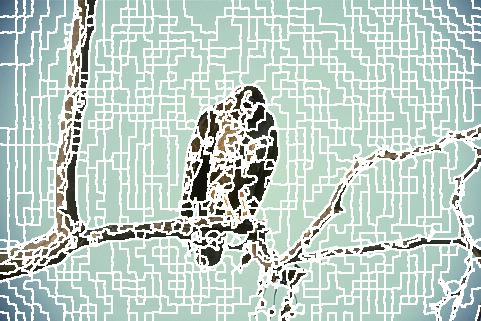
\includegraphics[width=\textwidth]{images/asari/ASARI/BSDS500/42049}
        \caption{Image 42049 de BSD. Nombre de superpixels : $472$. Taux d'erreur de sur-segmentation : $\nombre{0,03}$. \modif{Taux de rappel sur les contours} : $\nombre{0,99}$.}
        \label{fig:asari-BSDS500-1}
        \end{subfigure}
        ~
       \begin{subfigure}[t]{0.4\textwidth}
      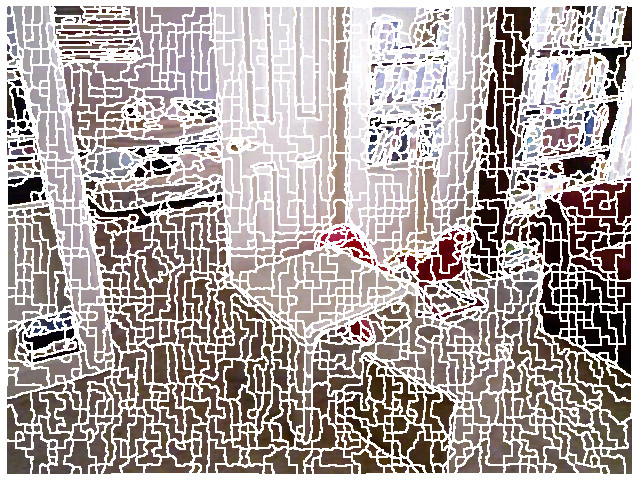
\includegraphics[width=\textwidth]{images/asari/ASARI/NYU/00001315}
        \caption{Image 00001315 de NYU. Nombre de superpixels : $905$. Taux d'erreur de sur-segmentation : $\nombre{0,07}$. \modif{Taux de rappel sur les contours} : $1$.}
        \label{fig:asari-NYU-1}
        \end{subfigure}
        \caption{Exemples de résultats obtenus par ASARI sur les bases de données BSD et NYU.}
        \label{fig:asari:BSD-NYU}
\end{figure}


\subsubsection{Résultats obtenus avec HSID}

Les résultats obtenus par ASARI sur la base de données HSID sont donnés dans le \modif{tableau~\ref{tab:res-hsid}}. Avec $1528$ superpixels \modif{en moyenne}, ASARI obtient le meilleur score d'adhérence aux contours. L'écart est significatif par rapport aux méthodes :
\begin{itemize}
\item de Vedaldi \textit{et al.}, $+4\%$ avec $1100$ superpixels en moins ;
\item de Rubio \textit{et al.}, $+15\%$ avec $300$ superpixels en moins ; 
\item de Conrad \textit{et al.}, $+24\%$ avec $500$ superpixels en moins ;
\item de Machairas \textit{et al.}, $+10\%$ avec $500$ superpixels en moins.
\end{itemize} 

La différence sur le score d'adhérence aux contours est moins important avec les méthodes de Felzenszwalb \textit{et al.} ($+ 1\%$) et d'Achanta \textit{et al.} ($+ 2\%$), mais le nombre de superpixels reste significativement inférieur avec, respectivement, $500$ et $300$ superpixels de moins. Enfin, ASARI obtient un score \modif{$\mathcal{F}_{FRC}$} identique à celui de l'algorithme de Liu \textit{et al.} en produisant $150$ superpixels de moins. 


\begin{table}[H]
\centering
\caption{Valeurs moyennes pour la mesure floue d'adhérence aux contours (\modif{$\mathcal{F}_{FRC}$)} et nombre moyen de superpixels par image (\modif{$N_{\mathbb{S}}$}), avec les données de référence HSID.}
\begin{tabular}{| l  |  l | l |}
\hline
 \cellcolor{gris}{Méthodes} &  \modif{$\cellcolor{gris}{\mathcal{F}_{FRC}}$} & \modif{$\cellcolor{gris}{N_{\mathbb{S}}}$}\\
\hline
Vedaldi \textit{et al.} & $\nombre{0,57}$ & $2583$ \\
\hline
Felzenszwalb \textit{et al.}  &  $\nombre{0,60}$ & $1998$ \\
\hline
Liu \textit{et al.} & $\nombre{0,61}$ & $1700$\\
\hline
Achanta \textit{et al.} & $\nombre{0,59}$ & $1854$  \\
\hline
Rubio \textit{et al.} & $\nombre{0,46}$ & $1881$\\
\hline
Conrad \textit{et al.} & $\nombre{0,37}$ & $2025$ \\
\hline
Machairas \textit{et al.}  & $\nombre{0,51}$ & $2069$ \\
\hline
ASARI  & $\nombre{0,61}$ & $1528$ \\
\hline
 \end{tabular} 
\label{tab:res-hsid}
\end{table}

La figure \ref{fig:asari-HSID} montre deux exemples de segmentations produites par ASARI sur les images de la base de données HSID. La figure \ref{fig:asari-HSID-1} est un autre exemple du caractère adaptatif d'ASARI, avec des superpixels capables de s'adapter à la taille des différents objets.  Sur la figure \ref{fig:asari-HSID-2}, l'information de texture permet de séparer l'objet principal du fond, pourtant de couleurs similaires.

\begin{figure}[htb]
        \centering
           \begin{subfigure}[t]{0.4\textwidth}
        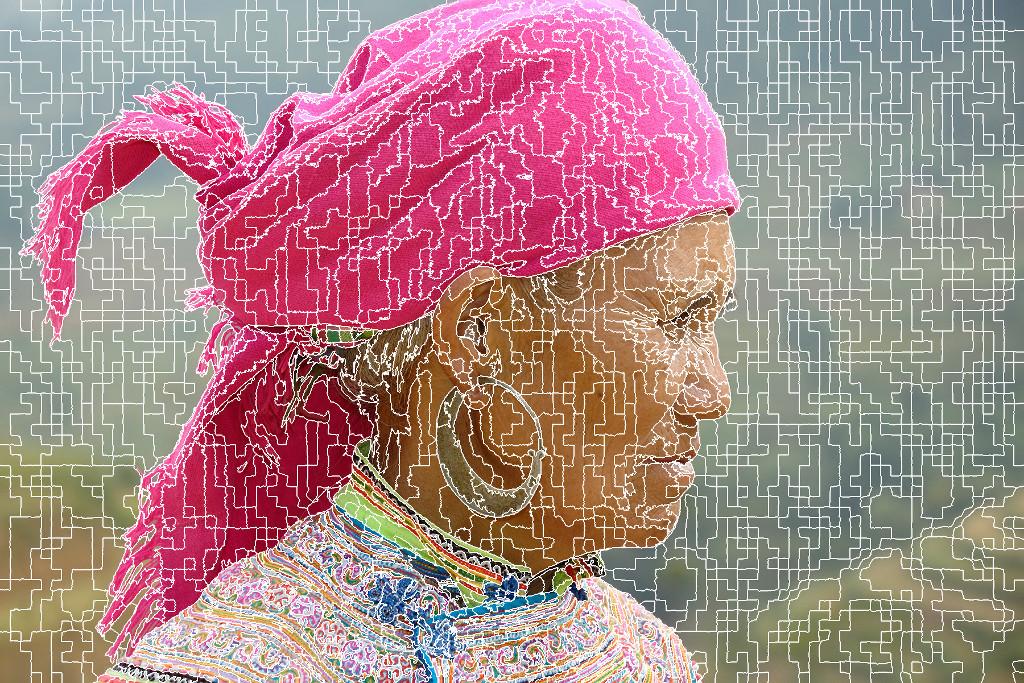
\includegraphics[width=\textwidth]{images/asari/ASARI/HSID/img-010}
        \caption{Image img-010. Nombre de superpixels : $1445$. Score d'adhérence aux contours : $\nombre{0,66}$.} 
        \label{fig:asari-HSID-1}
        \end{subfigure}
        ~
           \begin{subfigure}[t]{0.4\textwidth}
        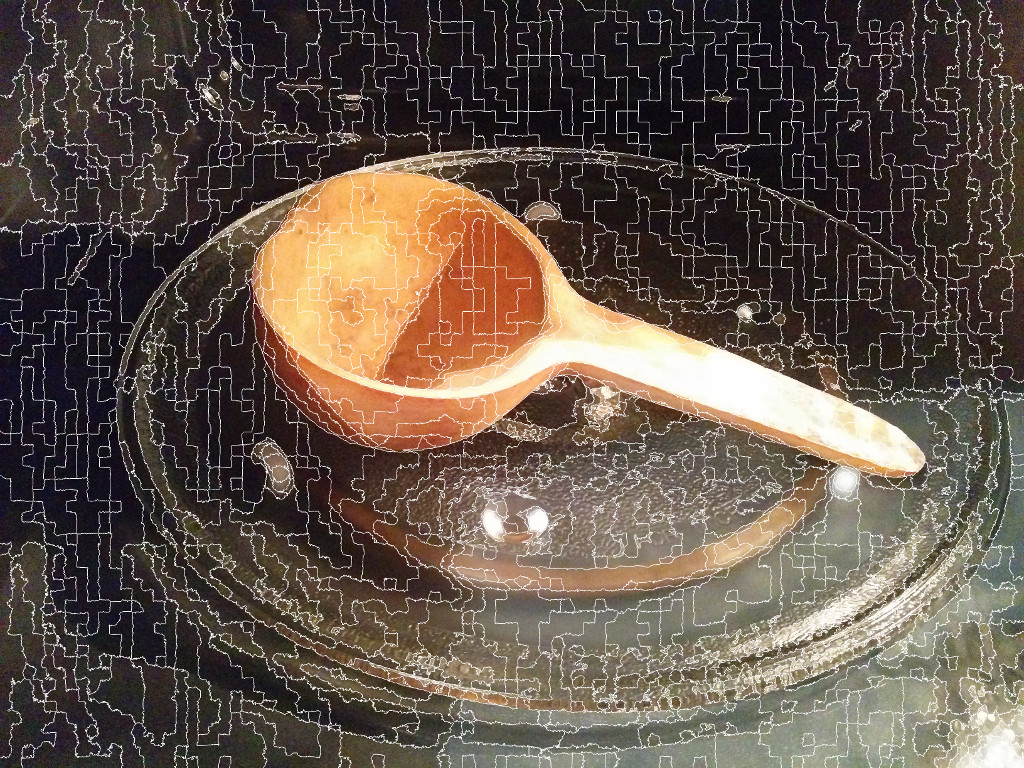
\includegraphics[width=\textwidth]{images/asari/ASARI/HSID/img-036}
        \caption{Image img-036. Nombre de superpixels : $928$. Score d'adhérence aux contours : $\nombre{0,61}$. }
        \label{fig:asari-HSID-2}
        \end{subfigure}
        \caption{Deux résultats obtenus par ASARI sur la base de données HSID.}
        \label{fig:asari-HSID}
\end{figure}




\subsection{Temps de calcul}

Les temps d'exécution moyens nécessaires à l'obtention des résultats précédents, pour chacun des ensembles de données de \modif{référence} sont donnés dans le tableau \ref{tab:asari:time}.

\begin{table}[h]
\caption{Temps d'exécution moyens en secondes pour chacune des bases de données.}
\centering
\begin{tabular}{| l  |  l | l |  l |}
\hline
 \cellcolor{gris}{Méthodes} &   \cellcolor{gris}BSD &  \cellcolor{gris}NYU &  \cellcolor{gris}HSID\\
\hline
Vedaldi \textit{et al.} & $1,24$  & $1,24$ & $79$ \\
\hline
Felzenszwalb \textit{et al.}  &  $0,10$ & $0,1$ & $10$\\
\hline
Liu \textit{et al.} & $1,11$ & $2,21$ & $36$\\
\hline
Achanta \textit{et al.}  & $0,09$ & $0,17$ & $3$ \\
\hline
Rubio \textit{et al.} & - &- & $37$ \\
\hline
Conrad \textit{et al.}  & $0,9$ & $1,19$ & $23$ \\
\hline
Machairas \textit{et al.}  & -& - &$29$ \\
\hline
ASARI  & $1,38$ & $2,89$ & $6$ \\
\hline
 \end{tabular} 
 \label{tab:asari:time}
\end{table}


Pour de petites images (BSD et NYU), ASARI est plus lent que les méthodes de l'état de l'art. En revanche, lorsque des images de grande taille comme celle d'HSID doivent être sur-segmentées, ASARI obtient des temps d'exécution significativement inférieurs à la quasi-totalité des méthodes avec :
\begin{itemize}
\item $73$ secondes de moins que l'algorithme de Vedaldi \textit{et al.} ;
\item $4$ secondes de moins que l'algorithme de Felzenszwalb \textit{et al.} ;
\item $30$ secondes de moins que l'algorithme de Liu \textit{et al.} ;
\item $31$ secondes de moins que l'algorithme de Rubio \textit{et al.} ;
\item $17$ secondes de moins que l'algorithme de Conrad \textit{et al.} ;
\item $23$ secondes de moins que l'algorithme de Machairas \textit{et al.}.
\end{itemize}

La seule méthode plus rapide qu'ASARI est l'algorithme SLIC d'Achanta \textit{et al.} qui produit une sur-segmentation en seulement $3$ secondes.

\section{Conclusion}
\subsection{Bilan par rapport à l'état de l'art}
Les évaluations que nous avons menées montrent que sur de petites images, semblables à celles qui composent les données de référence des ensembles BSD et NYU, le bénéfice d'ASARI par rapport à l'état de l'art est ténu. Ces résultats s'expliquent par deux phénomènes :
\begin{itemize}
\item les mécanismes visant à réduire la complexité algorithmique d'ASARI ont un impact moindre, ce qui contribue à augmenter l'écart entre les temps d'exécution de cet algorithme et ceux des méthodes concurrentes ;
\item la petite taille des images implique que les pixels à partager entre les régions de $V_{0}$ sont peu nombreux. En particulier, il est difficile de fixer la taille de ces dernières de manière à ce que le nombre de pixels les composant soit suffisamment élevé pour le descripteur de texture mais suffisamment faible pour éviter d'introduire des erreurs de sur-segmentation \modif{dès} cette étape.
\end{itemize}
Ajoutons que l'une des contreparties du fait qu'ASARI fusionne des régions réside dans le fait que, lorsqu'une arête est supprimée à tort, l'erreur commise est plus importante que pour des algorithmes travaillant au niveau du pixel.

Avec des images de grande taille, les avantages d'ASARI deviennent plus marqués. Nous constatons notamment que :
\begin{itemize}
\item avec la méthode de Liu \textit{et al.}, ASARI est le seul algorithme à atteindre un score d'adhérence aux contours de $\nombre{0,61}$ ;
\item les superpixels produits par ASARI sont significativement moins nombreux ;
\item en termes de rapidité d'exécution, ASARI obtient la deuxième place, avec seulement une durée moyenne de $6$ secondes, là où tous les autres algorithmes, à l'exception de SLIC, sont au delà des $10$ secondes.
\end{itemize}

Le code source d'ASARI a été mis à disposition\footnote{\url{http://image.ensfea.fr/asari/}}.

\subsection{Perspectives}
Malgré ces résultats encourageants, nous ne pensons pas qu'ASARI puisse être, dans l'état actuel, intégré de manière fructueuse à $S \alpha F$. Les deux principaux problèmes sur lesquels nous souhaitons poursuivre nos travaux concernent :
\begin{itemize}
\item la diminution des erreurs commises pour les petites images ;
\item la réduction du temps d'exécution. 
\end{itemize}

Afin d'améliorer les performances d'ASARI sur les ensembles de données BSD et NYU, nous réfléchissons à l'introduction de mécanismes permettant de remettre en cause l'intégrité d'un sommet et de pouvoir le séparer en plusieurs régions. Nous envisageons la prise en compte d'une information sur les contours et recherchons un procédé capable de répartir de manière efficace les pixels d'une région en plusieurs sous-ensembles connexes.

Dans l'optique de réduire les temps d'exécution\modif{,} nous travaillons actuellement à identifier les étapes d'ASARI les plus coûteuses, afin d'en réduire la durée, soit en parallélisant ces parties de l'algorithme, soit en recherchant une approximation des informations calculées.

Si ces deux pistes s'avèrent fructueuse, ASARI permettra sans aucun doute d'améliorer la méthode de segmentation interactive $S \alpha F$.